\section{Reflections on our process}
In \autoref{sec:our-process} we described our process and the things that we used from scrum.
In this section we reflect on our process, the changes that we had done throughout the semester as well as what we would change for our future projects.

\subsubsection{Scrum}
Our scrum inspired process worked well with sprints, sprint planning, sprint backlog, product owner, Scrum Master, planning poker, product backlog and product increment.
We took turns on having the role as PO and scrum master.
The PO/Scrum Master had the task of planning the next product backlog and add a DoD (definition of done) onto every task in the product backlog.
This person also had the responsibility to send material to the supervisor, book a conference room and responsible for the planning poker.
The sprint backlog and product backlog can be seen on \autoref{fig:trello-kanban}. 
The leftmost column is the product backlog, the next four column are the sprint backlog.
These are split into \textit{Sprint Backlog}, \textit{In progress}, \textit{In review} and \textit{Done}.
This gives us a better overview on how far people are with their tasks.

\begin{figure}[H]
    \centering
    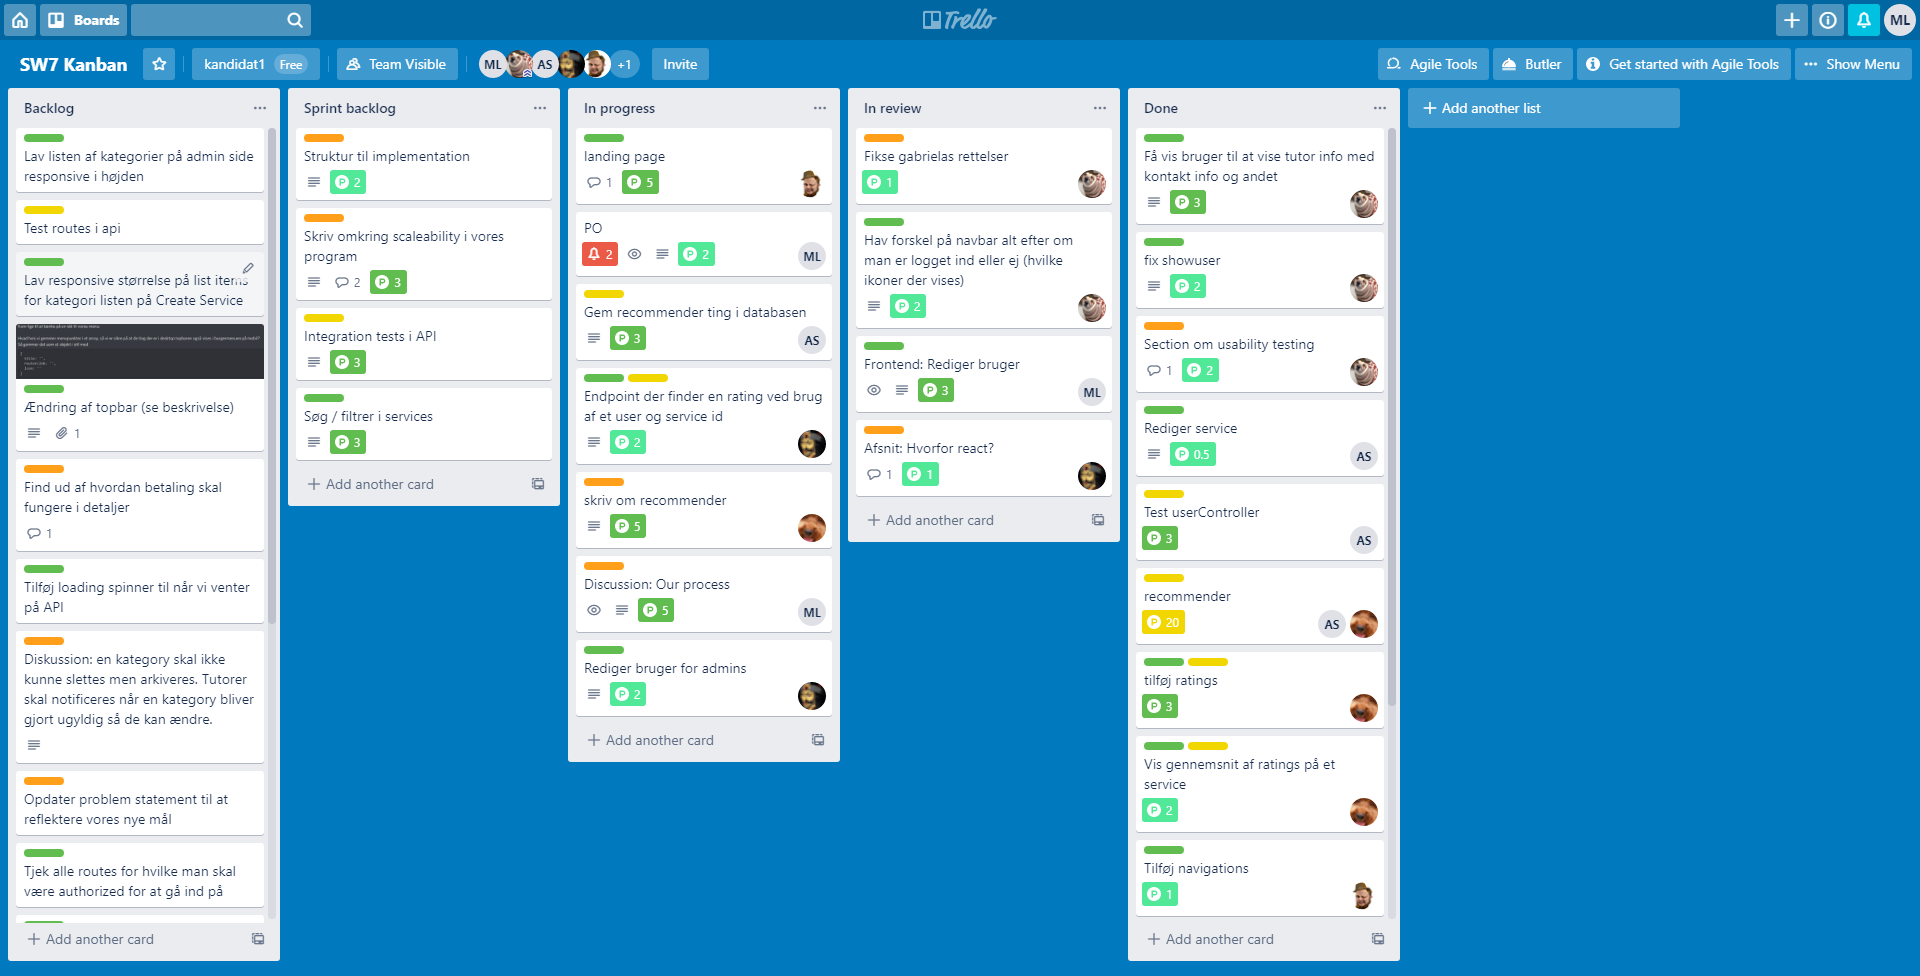
\includegraphics[width=0.8\linewidth]{figures/trellopicture.PNG}
    \caption{Our kanban board for the product and sprint backlog on Trello}
    \label{fig:trello-kanban}
\end{figure}
\noindent
When we conducted the sprint planning, we would use planning poker to estimate how many story points each task should have and then the persons with the highest and lowest story points would discuss the reasoning behind it.
The story points were often very different if there were ambiguities, and people understood the tasks differently.
This gave everyone the same understanding on how the given tasks should be solved and eliminate most ambiguities. 
\\
However, later in the project when we started to develop the application and learning \textit{React}, it started to become less systematic.
This was often due to it being difficult to estimate how long each task would take to solve.
\\\\
We also stopped conducting the retrospective meetings. 
This could have helped making the project more structured as we could have discussed the problems that we faced and the reasons why we did not complete our tasks in time.

\subsubsection{Formal reviews}
The formal reviews was something that we changed in the middle of the semester, so that two people had to review a pull request together and not individually.
Formal reviews were described in \autoref{sec:formal-reviews}.
The first hour of every workday was spent on reviewing pull requests.
\\\\
This increased the quality of the pull requests, as more errors were caught when two people had to debate the code.
This is however more time consuming and more difficult to plan.
If two people are in process of reviewing a pull request another person can be waiting for them to finish if they are assigned a pull request with one of them. 
Then when a pull request have been reviewed and if changes are requested, then these people have to come back to review the changes.
To make this more organized a we created a PR spreadsheet to give an better overview of which pull requests you are assigned to, and who are currently requested to do many or few reviews.
This can be seen on \autoref{fig:formal-reviews}.
\begin{figure}[H]
    \centering
    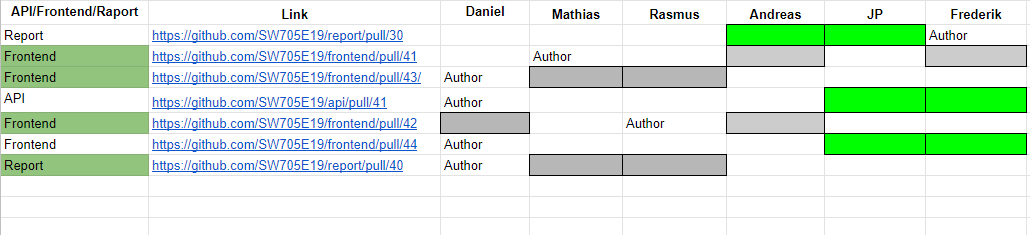
\includegraphics[width=\linewidth]{figures/formal-reviews.PNG}
    \caption{Pull request assignment sheet.}
    \label{fig:formal-reviews}
\end{figure}

\subsubsection{Working from home}
Unlike other semesters, we were not assigned a group room this semester.
This resulted in us working from home most days in the week, because we thought this would be easier and as productive as if we met on the university.
One of the cons of working from home is that it is more difficult to get help from the other group members and this can lead people to get stuck on tasks.
After a few weeks we realized that it would be better if we had one workday together every week.
This was really beneficial as the more experienced React developers were able to help other members that were less experienced.
It was also easier to conduct a sprint planning when we met in person.

\subsubsection{Supervisor meetings}
The day before the supervisor meeting we sent the report, a reading guide and an agenda for the meeting.
Our supervisor gave feedback on the material that we sent to her and during the meeting we presented the things that we had done the previous week.
These meetings have been longer than the meetings we had previously experienced in last semesters, but this also resulted in better feedback, as the questions she asked made us reflect on certain choices we had made.

\subsubsection{What we would do differently}
One of the problems that we faced was that people could get stuck on tasks.
For future projects we would try to be more aware of where people are in the process, so that it would be easier to help them with solving their tasks.
One of the solutions to this could be daily standups, so that we are aware of where people are with their tasks, and which once they have not completed.

Another solution could be to have more workdays on the university, so that people have an easier time getting help from one another.
It is especially important in the beginning of the semester when there are still a lot of ambiguities and uncertainties with the project.  
